% ----------------------------------------------------------------------------------------
% This contains all the content under Part: Hardware
% ---------------------------------------------------------------------------------------
\part{Hardware}
\chapter{Hardware Architecture}
\label{chap:partHwHwArch}
\section{Static Vs. Dynamic Power}
A hardware architect will almost always face a tradeoff between area of a module and its clock frequency\marginnote{Static power consumption is because of leakage; Dynamic because of transistor toggling}. For instance, an FIR filter with 10 taps with a max throughput of 48 KHz can either be implemented with 10 single-cycle multipliers or with a single single-cycle multiplier. The former choice would mean that the filter would have to be clocked at 48 KHz and the latter would imply a clocking of 10*48 KHz. This area vs. clock tradeoff is essentially a static vs. dynamic power consumption tradeoff. Though there are no fixed formula on how to decide one over the other, the thumbrule is to conserve area and increase clock frequency up to 500 MHz. 

\section{Choosing to Go the Hardware Way}
Any functionality can be implemented in software or hardware. Each has its own advantages. Software is very flexible in that something broken can easily be fixed, whereas hardware is pretty much written in stone. However, software uses the CPU's generic functionalities, and hence, will most likely consume higher power compared to a hardware tailored for one particular functionality\marginnote{SW is flexible; HW is efficient}. However, when the use case requiring the functionality in question is over, CPU's MHz can be utilized for some other functionality, while the hardware will be sitting idle leaking power - So if the functionality in question isn't alive most of the time, implementing it in hardware may be a bad idea. Hence, \marginnote{Thumbrule is to go HW for ASICs, go SW for general purpose ICs}hardware accelerators are usually the way to go in ASICs, such an ADSL system where the same kind of functionality needs to be repeated for every received symbol. And they are usually \emph{not} the way to go in general purpose computing devices such as application processors, where it is hard to predict when a certain functionality (as part of a use case) will be alive and when it won't be alive. 

These above described scenario, of course, \emph{usually} the case in general purpose ICs, which means there are unusual cases where hardware may be the way to go even when the functionality in question occurs rarely\marginnote{All thumbrules have caveats!}. An example would be a system where we don't know what are all the software that can run on the CPU . In this case, if we implement all the known functionalities in hardware, then CPU MHz will be freed up to run the unknown functionalities. Another example would be a CPU that would run at SV voltage corner at, say 500 MHz, and would be pushed to the HV corner if a 50 MHz functionality is added to it - If the power rail the CPU is connected to has all of its other components asking mostly for SV, then the power rail would now have to run at HV just because of the CPU. This may cause higher leakage in all other components - let us call this unnecessary extra leakage in other components as \(\Delta P_a*T_f\), where $\Delta P_a$ is the extra leakage power and $T_f$ is the time for which the functionality in question will be alive. Keeping this in one hand, suppose we use a hardware module to implement that 50 MHz functionality in question and if the unnecessary leakage power of the module when the functionality is not alive is \(\Delta P_b*(T_b-T_f)\), where $T_b$ is some sort of a total time for all  use cases. If \(\Delta P_b*(T_b-T_f) < \Delta P_a*T_f\), then it would make sense to implement that 50 MHz functioanlity in hardware.

Besides the power angle, there is also a latency angle that needs to be considered - software will always work on chunks of data at a time, while hardware can work on a sample-by-sample basis\marginnote{HW can operate sample-by-sample; SW only on chunks}. This is because the OS allocates time slices to different software codes in chunks and within that chunk, it is economical to process data in chunks as well. This automatically means higher running latency. So hardware usually has lower running latency than software. This, of course, doesn't apply to hardware modules that cannot operate on data on a sample-by-sample basis. An example is an FFT accelerator. 

\chapter{Miscellaneous}
\label{chap:partHwMisc}
\section{Memory}
There are two types of memory namely volatile and non-volatile memory. As a thumbrule, non-volatile memory is slower (in reading, writing) than volatile memory. Within volatile memory, there are two sub-types namely Static RAM (SRAM) and Dynamic Ram (DRAM).  DRAM uses a trasistor and a capacitor to store a bit, while an SRAM uses a flip-flop containing 4 to 6 transistors to do the same job. Thus a DRAM has a higher memory density (more bits per sq. mm) than SRAM. The downside of DRAM is that it is slower to read, write than SRAM \marginnote{SRAM for speed; DRAM for memory density} and also needs to be constantly ``refreshed'' because the capacitor slowly leaks its charge. Usually on-chip RAMs, small in size, such as scratch pad RAMs and Caches are SRAMs, while the ``main memory'', relatively much larger in size, is a DRAM and is off-chip. The SoC, however, provide a ``Memory Controller'' that can periodically refresh (and do many other things) the off-chip DRAM. 

	\begin{figure}[h!]
	\centering
	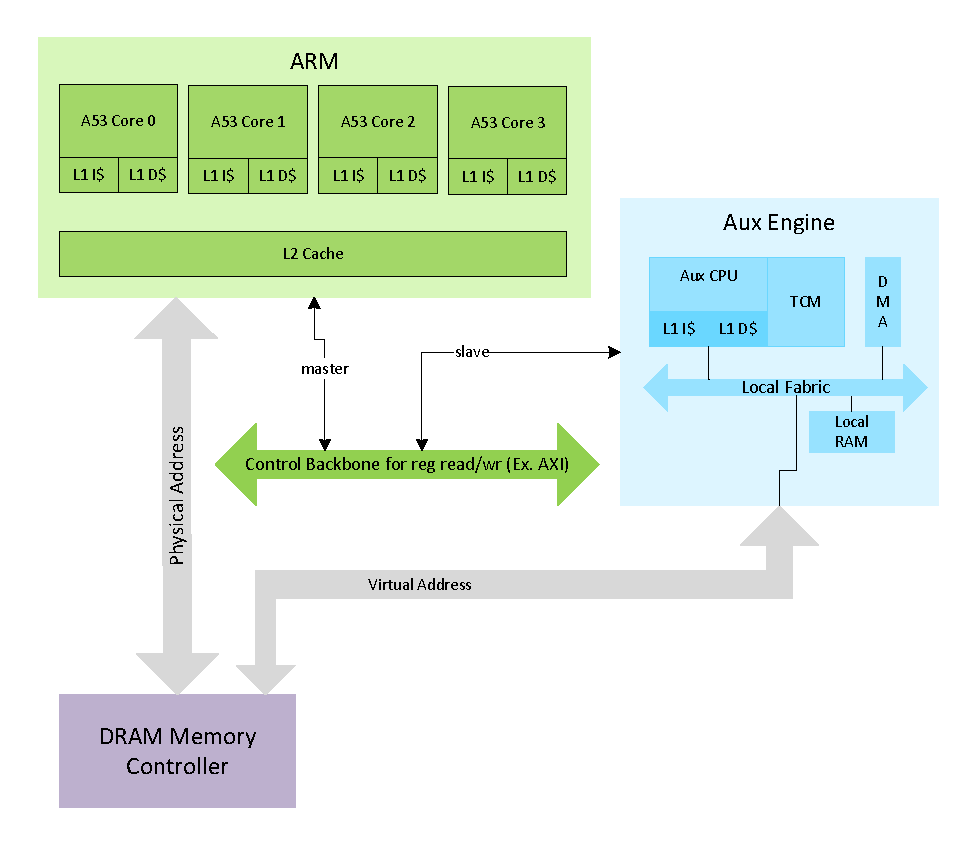
\includegraphics[width = \textwidth]{partHW/Memory}
	\caption{Different Memory Types}
	\label{fig:mem}
	\end{figure}
	
The term ``Tightly Coupled Memory'' is used for scratch RAMs that CPUs have dedicated access to - i.e., RAMs that aren't shared with other modules\marginnote{TCMs are SRAMs dedicated to CPU}. Thus RAMs sitting on a bus (say AXI) as a slave serving many bus masters (say, a CPU, a DMA engine etc.) cannot be termed as a TCM. By design, CPU access to TCMs is faster than access to other internal RAMs as the CPU will have to deal with bus protocol overheads and has to compete with other modules while trying to access a non-TCM RAM. The downside of this is that TCMs may be under-utilized (for ex., when CPU is in WFI), and hence it should be economically sized to have the smallest memory capacity acceptable.

Cache, like TCM, is a memory that is dedicated to the CPU. It is used to store copies of frequency accessed data that is present in some iRAM (on or off-chip). When a CPU starts afresh (say, after a reset), and tries to read a memory location, instead of reading the value in the location, a DMA is started to copy an entire block of memory in the vicinity of the generated address from the RAM to the Cache. The idea is that the CPU is running a code that is likely to access nearby address locations in that block sometime in the near future. Any further CPU access to addresses inside the block will imply reading data from the Cache instead of going all the way to the RAM. An importnat point to note is that, when the first DMA happens, the DMA first fetches the address CPU asked, no matter whether the address is at the beginning of the block to be fetched, or at the end of it or somewhere in the middle. This means that CPU will quickly get the data it wanted and will start working on it, while, in parallel, the DMA will continue fetching the remainder of the block. 

Just like the OS loads a program from a flash memory into RAM before executing it, - because flash access is slower than RAM - one can think of Cache as a kind of a TCM into which contents of the RAM are loaded into so that access to the contents could be faster. However the similarities end there. While OS deliberately loads a code from flash into RAM, is managed completely by hardware and done dynamically (per memory access) rather than just once before a context switch. For instance, the first time CPU accesses a location, it results in what is called a \emph{cache miss}, which means that the data CPU is trying to access is not in cache, but need to be copied into cache from RAM. After the first DMA is over, when the next addresses CPU accesses are found to be in the cache, it is called a \emph{cache hit}. Since cache is limited, a future cache miss may mean that current contents of the cache may have to be flushed in order to make way for new contents. All of these tasks are part of the cache hardware and are performed dynamically.  More details about how cache works, various cache architectures can be found in the Cache \& MMU section in \nameref{chap:upArch}

	\begin{highlightedText}
	\begin{tabular}{l r}
		Memory Size : & Dynamic RAM > Internal RAM > L2 Cache > L1 Cache\\
		Speed : & Dynamic RAM < Internal RAM < L2 Cache < L1 Cache\\
	\end{tabular}
	\end{highlightedText}

\section{Hard Reset and Soft Reset}
Hard reset is used to reset a modules registers back to their ``Power-on Reset (POR)'' values and reset internal state machine to the initial state. Soft reset does only the latter part of resetting the state machine while the register values (had they been modified by the software) are not reset back to their default values\marginnote{Hard reset affects reg values. Soft reset doesn't}. Generally the hardware architect defines what the POR values should be for every register field. The POR value is then converted into necessary pull-ups and pull-downs\footnote{``Pullups'' and ``pulldowns'' are resistors connected to Vcc and Gnd respectively} sitting behind a mux that either forces these values (on hard reset) or allows user writes through. The pull-ups and pull-downs do occupy space and one may be tempted not to define the POR value (leave it at X): After all, the POR values are prescribed so as to reduce SW configuration burden, and if the HW architect chooses, s/he could make it mandatory for the software to always configure all the registers of a module before using that module, and hence save area by eliminating pull-ups and pull-downs. However this is a bad idea as the possibility of having a bit as X, at any time, implies X propagation and verification engineers now have to identify all the conditions when this X could happen and all the paths in the module this X could be propagated to and manually waive them in the testing tool. This process is cumbersome. Besides that, not having POR values is just a bad idea - it is akin to having variables in a software that come up with garbage values: if the code accidentally utilizes such a variable without assigning a value, imagine the bugs that could spawn. 

\emph{A note on defining POR values}: POR values must be chosen with the big picture of the scenarios in which the module in question will be used. One cannot frivolously make the POR values to be all zeros\marginnote{It is idiotic to make all POR values zeros}. The idea is that, if we know the most likely configuration of the registers, then the POR values should match that configuration - so that, when SW wants to use the module after power-on or a hard reset, they can simply configure one or two registers (possibly just write to the enable register) and get on to using the module.

Hard reset is asynchronous in nature. So a module need not have its clock running when a hard reset is applied. But de-asserting a hard reset requires clock. So generally one turns on the power and clock of a module before hard-resetting it. Soft reset is completely synchronous. So pretty much every operation on a module requires the clock to be on first.


\chapter{Transistor Amplifier}
\section{Transistor Characteristics}
In a Bi-Junction Transistor (BJT), Collector is physically the largest region, followed by the Emitter. Base is the smallest region. In terms of doping, Emitter is the most heavily doped of the three, followed by the Collector and the Base is the least doped. The following picture captures this info. 

	\begin{figure}[h!]
	\centering
	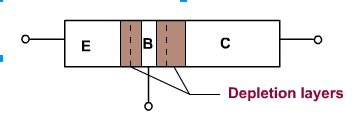
\includegraphics[width = 0.5\textwidth]{partHW/BJT_Regions}
	\caption{A BJT}
	\label{fig:bjt}
	\end{figure}

Let us look at how BJT acts as an electrically controlled switch in the CE configuration. We can use an abstract analogy for it: Imagine we are trying to turn right into Aakruti homes. But the gate is closed. We are waiting for the gate to be opened. There are lot of cars waiting behind us that need to continue going down the street - although the street is empty, they cannot go because we are blocking them. The moment the gate is opened and we make the turn, cars behind us can continue down the street. We can think of the Aakruti homes gate as the terminal connecting Base to the battery - as soon as it is positively biased, it is like opening the gate. This will allow electrons to smoothly from the Collector to the Emitter. 

In BJT, say, in an npn one, the way this analogy works is that, as soon as BE is positively biased, electrons in the depletion layer get dislodged and go out of the Base terminal thereby allowing electrons to flow from Emitter to the Collector \cite{sanghoKim16}. The reason why not all electrons will simply exit out of the Base terminal is that the Base is very thin and the path out of the Base is like a narrow gate - not many cars can turn into it - and since the wide road is now unblocked, most go from the Emitter to the Collector.

Let us look at some SPICE simulations and try to understand the transistor characteristics better. First let us understand the Base-Emitter diode's voltage and current characteristics by using the circuit in \autoref{fig:beDiode}. The Collector is intentionally left to float as we are only interested in the other two terminals. 

	\begin{figure}[h!]
		\centering
		\makebox[\linewidth][c]{
		\begin{subfigure}[b]{0.4\textwidth}
			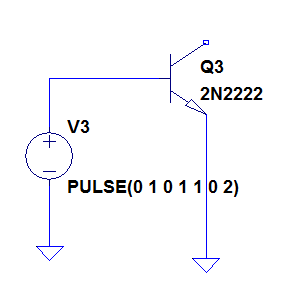
\includegraphics[width = \textwidth]{partHW/BE_Diode}
			\caption{BE Diode Circuit}
			\label{fig:beDiode}
		\end{subfigure}
		\begin{subfigure}[b]{0.7\textwidth}
			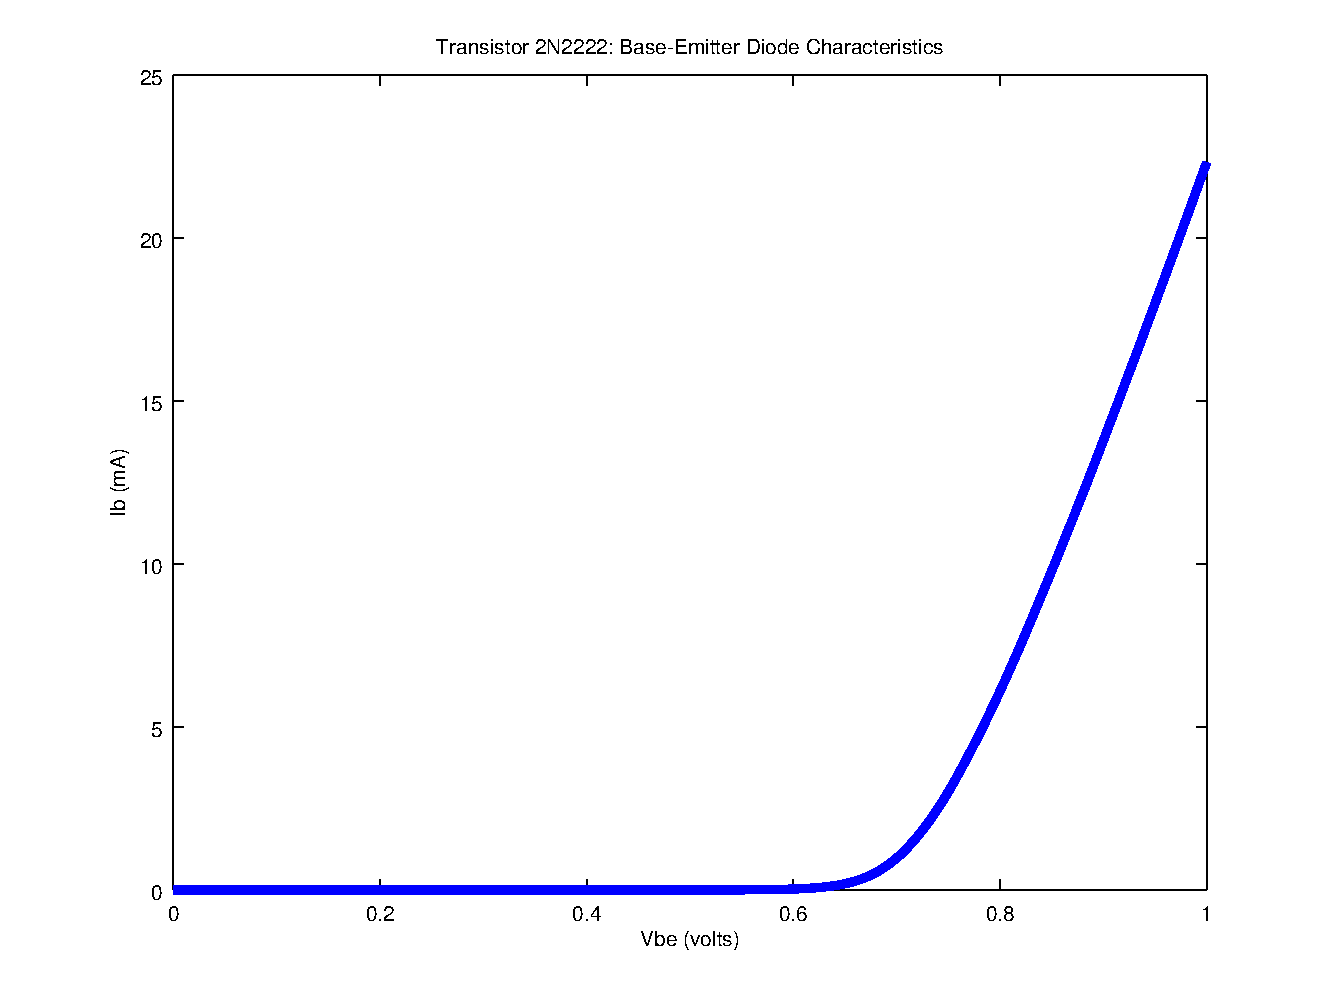
\includegraphics[width = \textwidth]{partHW/NPN_2N2222_Vbe_Ib}
			\caption{$V_{BE}$ Vs. $ I_B$}
			\label{fig:beDiodeCurve}
		\end{subfigure}
		}
		\vskip\baselineskip
		\makebox[\linewidth][c]{
		\begin{subfigure}[b]{0.85\textwidth}
			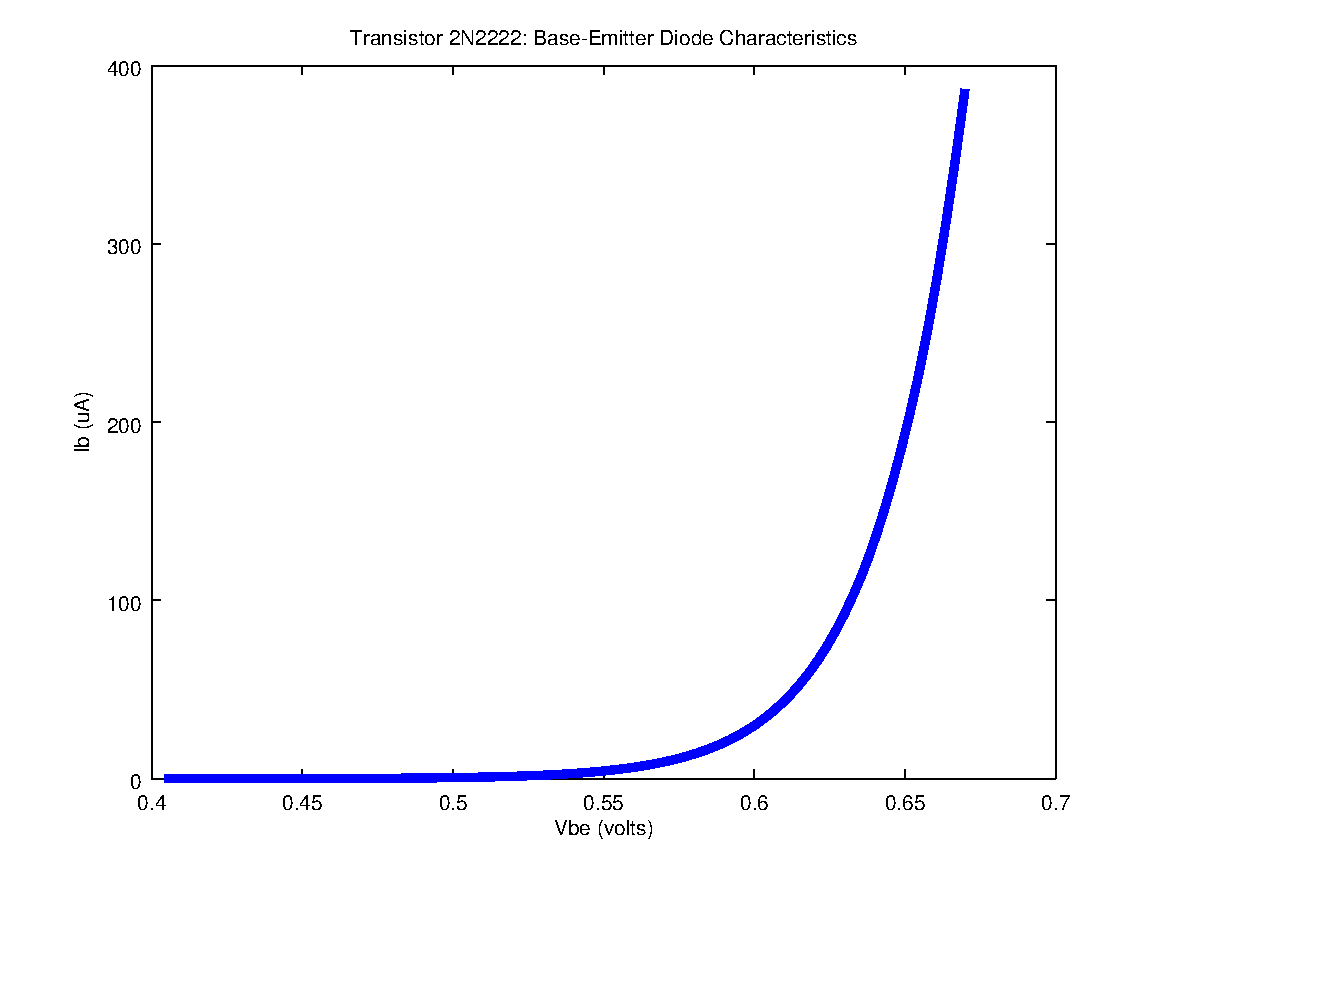
\includegraphics[width = \textwidth]{partHW/NPN_2N2222_Vbe_Ib_zoomed}
			\caption{$V_{BE}$ Vs. $ I_B$ Zoomed in}
			\label{fig:beDiodeCurveZoomed}
		\end{subfigure}
		}
		\caption{The Base-Emitter Diode}
		\label{collage:beDiode}
	\end{figure}

When we run the simulations and check the relationship between voltage and current at the Base-Emitter terminals, we get a graph as shown in \autoref{fig:beDiodeCurve}. A zoomed in version is shown in \autoref{fig:beDiodeCurveZoomed}



It is clear that the diode opens at around a $V_{BE}$ of 0.65V or so and from there on, it seems that $V_{BE}$ and $I_B$ are linearly related to each other. 

We made a small mistake in the circuit depicted in \autoref{fig:beDiodeCurve} - We gave a fixed voltage to the BE terminal. However, as we know, as the voltage is increased, the resistance across BE decreases. This is not captured in the circuit and the associated graphs. We can introduce a Base resistor so that, when the resistance across BE changes, $V_{BE}$ changes. \autoref{fig:beDiodeWithRb} shows this circuit and \autoref{fig:VbeIbVsVin}, \autoref{fig:VbeIbVsVin_zoomed} depict how $V_{BE}$ and $I_B$ change with $V_{in}$

           \begin{figure}[h!]
		\centering
		\makebox[\linewidth][c]{
		\begin{subfigure}[b]{0.4\textwidth}
			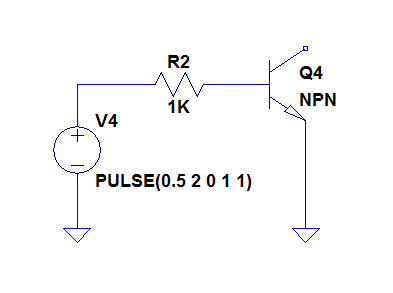
\includegraphics[width = \textwidth]{partHW/BE_Diode_With_Rb}
			\caption{BE Diode Circuit}
			\label{fig:beDiodeWithRb}
		\end{subfigure}
           	\begin{subfigure}[b]{0.7\textwidth}
			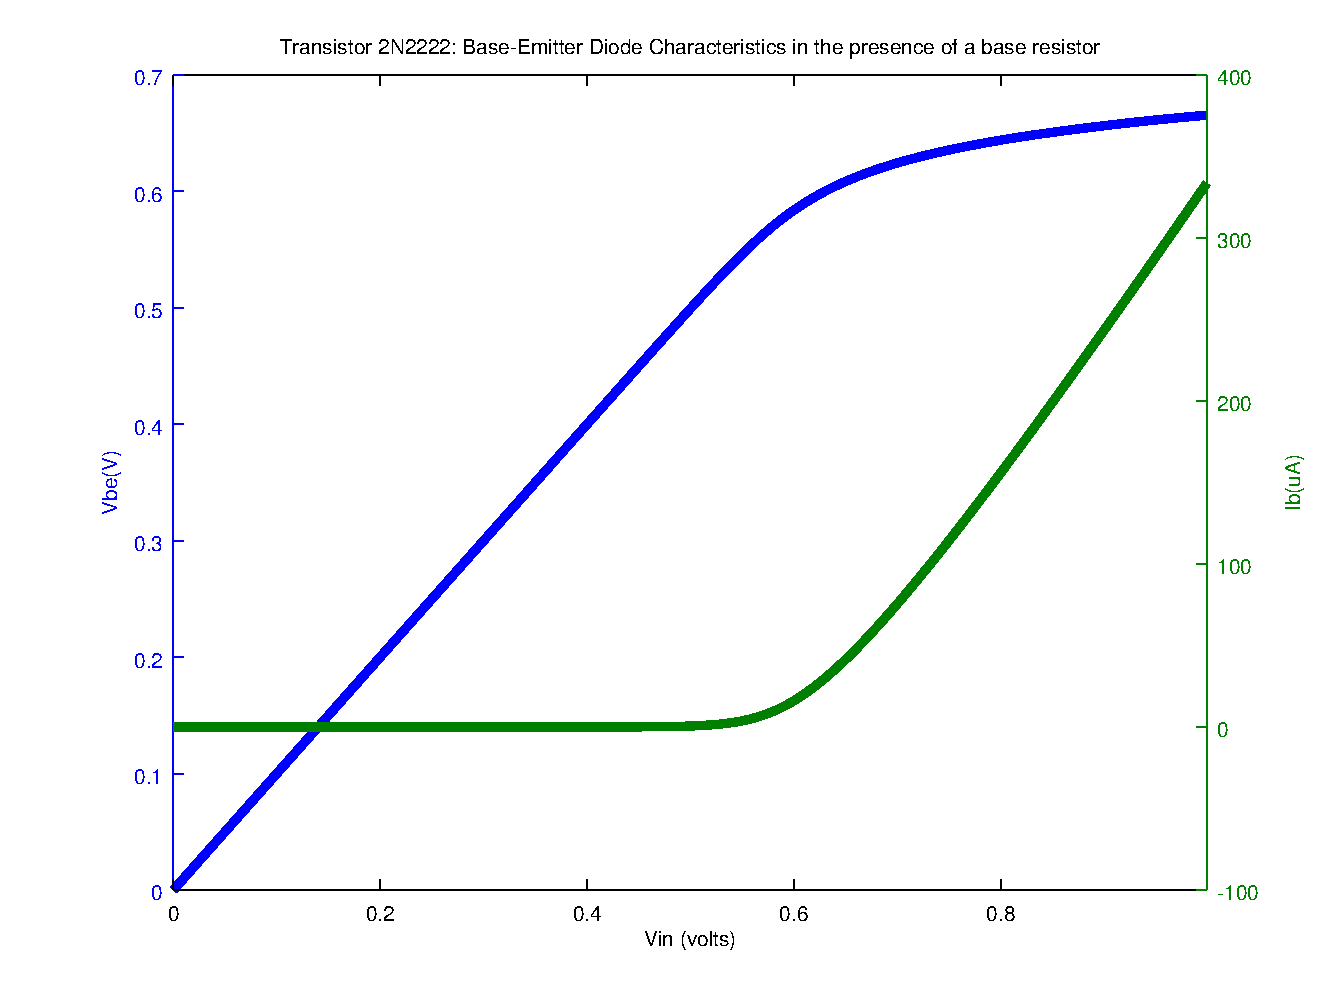
\includegraphics[width = \textwidth]{partHW/NPN_2N2222_Vin_Vbe_Ib}
			\caption{$V_{BE}$ Vs. $ I_B$}
			\label{fig:VbeIbVsVin}
		\end{subfigure}
		}
       		\vskip\baselineskip
		\makebox[\linewidth][c]{
		\begin{subfigure}[b]{0.85\textwidth}
			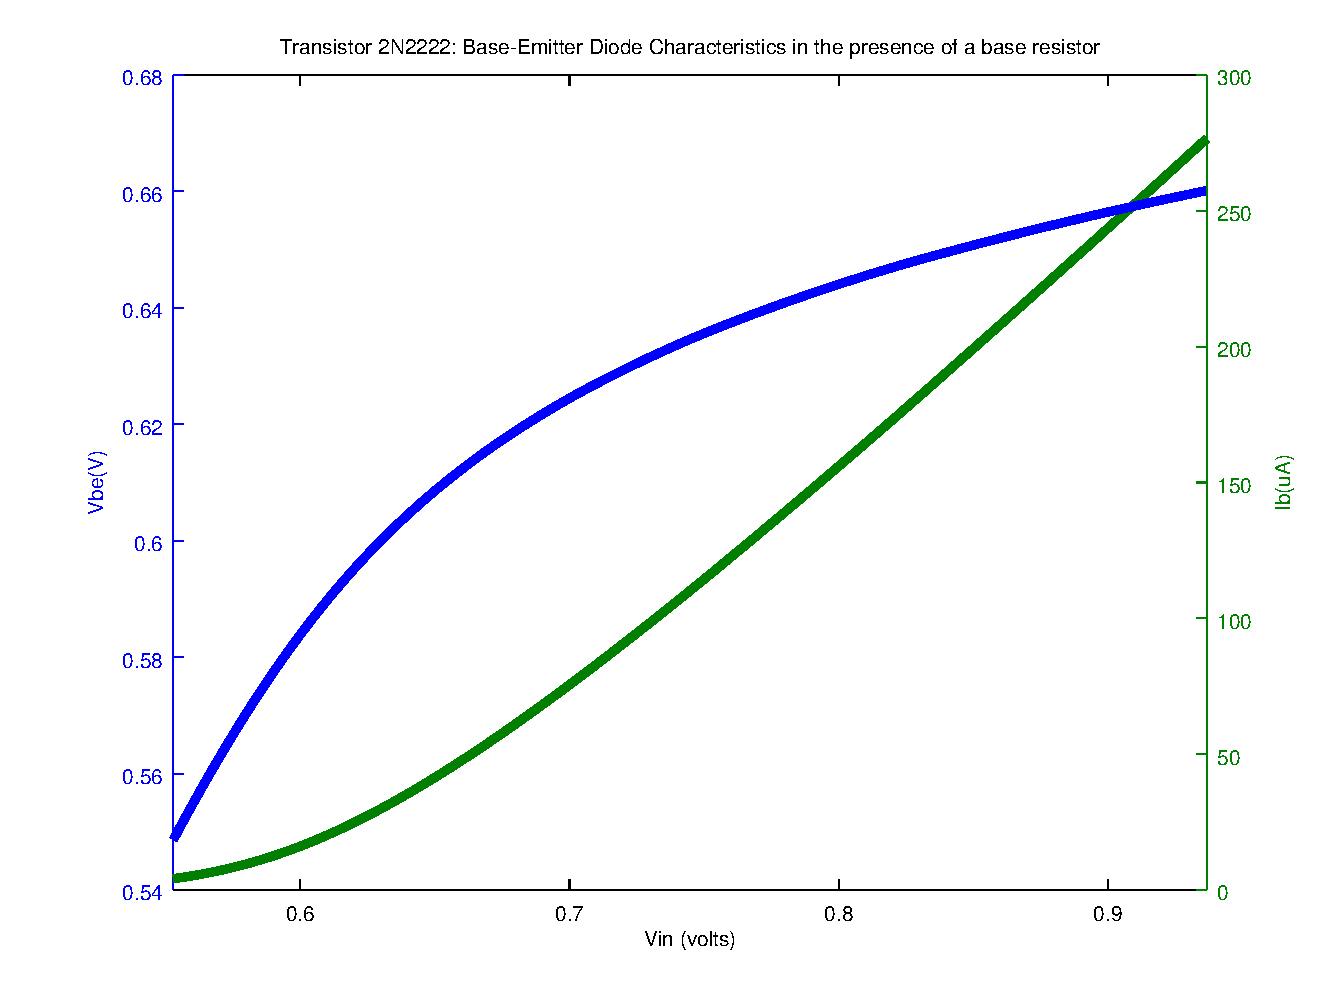
\includegraphics[width = \textwidth]{partHW/NPN_2N2222_Vin_Vbe_Ib_zoomed}
			\caption{$V_{BE}$ Vs. $ I_B$ Zoomed in}
			\label{fig:VbeIbVsVin_zoomed}
		\end{subfigure}
		}
		\caption{The Base-Emitter Diode with a Base Resistor}
		\label{collage:beDiodeWithRb}
	\end{figure}



Now, with the new figures, we can clearly see that $V_{BE}$ doesn't keep on increasing with $V_{in}$. After reaching about 0.66V (approx), $V_{BE}$ saturates. We can also see that $I_B$ is practically zero until $V_{BE}$ is around 0.6V and then increases almost linearly w.r.to $V_{in}$ after that. 

Now that we understand the BE diode well, we can move on to exploring the Collector side of things. We can do this by connecting the Collector to a voltage source as shown in \autoref{fig:transChar1}. A series resistor at the Collector is added for the same reason we added a series resistor at the Base.  

	\begin{figure}[h!]
		\centering
		\makebox[\linewidth][c]{
		\begin{subfigure}[b]{0.5\textwidth}
			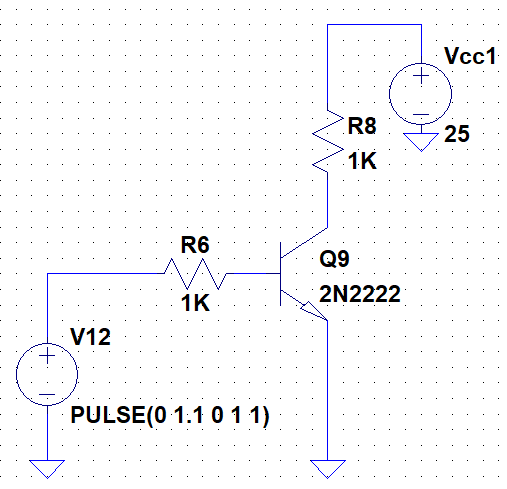
\includegraphics[width = \textwidth]{partHW/Transistor_BEC}
			\caption{Base-Emitter Vs Collector}
			\label{fig:transChar1}
		\end{subfigure}
		}
		\vskip\baselineskip
		\makebox[\linewidth][c]{
		\begin{subfigure}[b]{0.75\textwidth}
			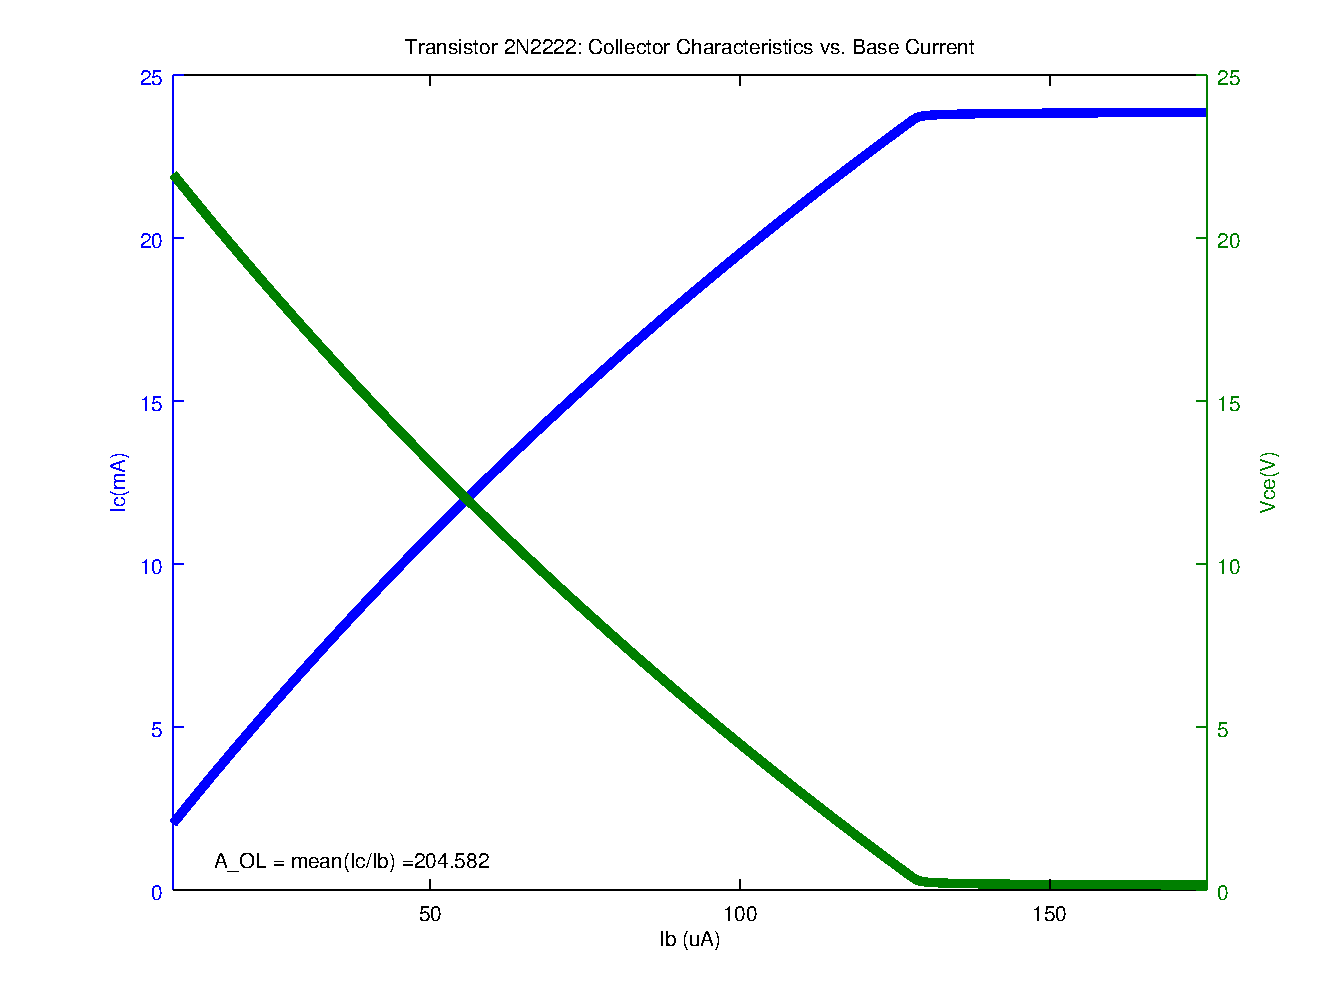
\includegraphics[width = \textwidth]{partHW/NPN_2N2222_Ib_Ic_Vce}
			\caption{$V_{CE}$, $I_C$ as functions of $I_B$}
			\label{fig:CollectorVsIb}
		\end{subfigure}
		\begin{subfigure}[b]{0.75\textwidth}
			\centering
			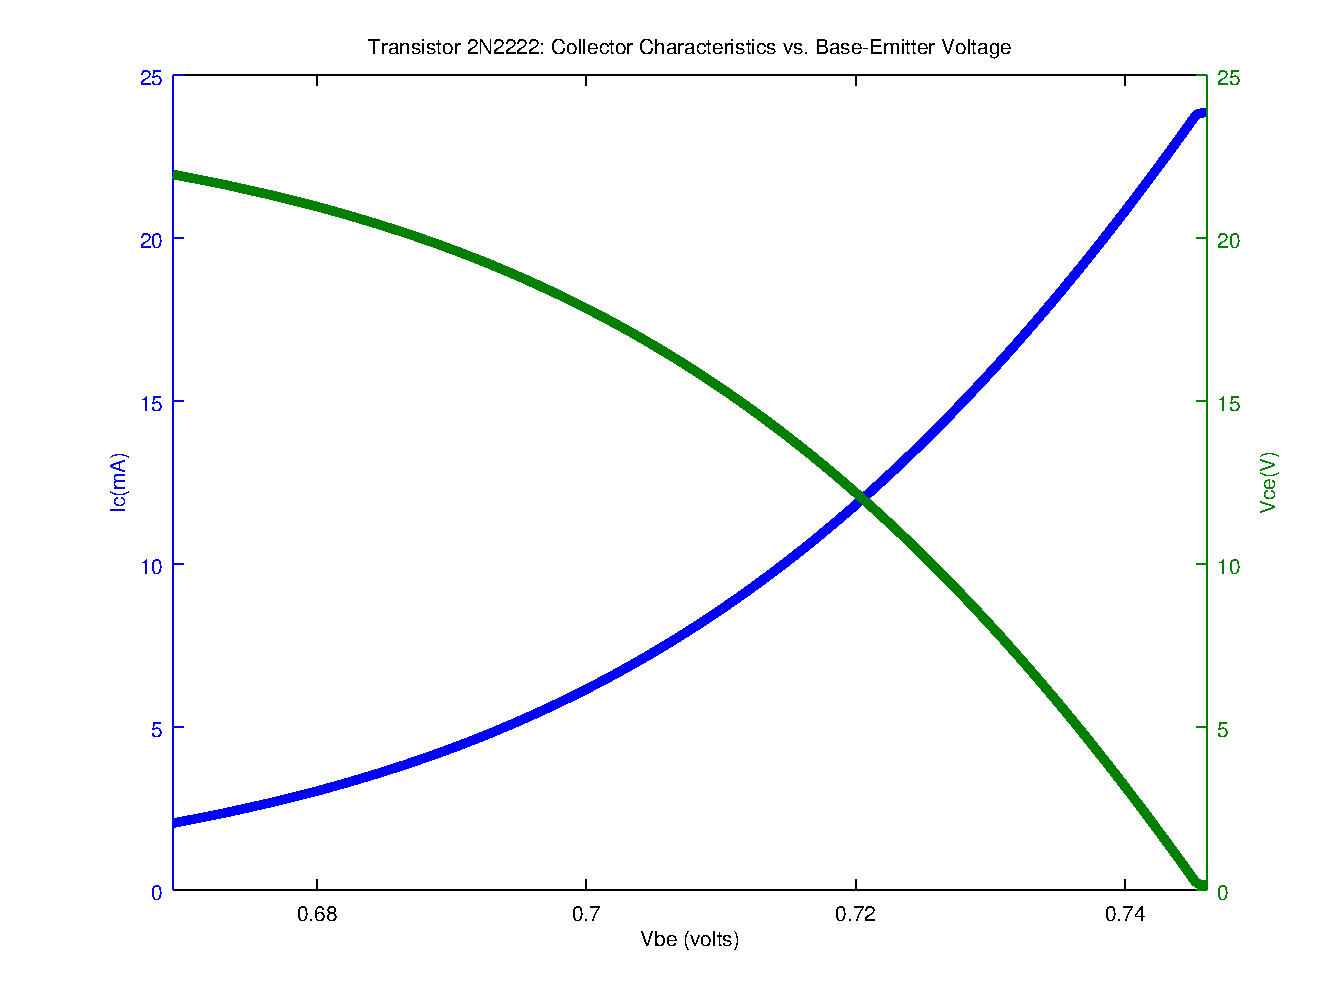
\includegraphics[width = \textwidth]{partHW/NPN_2N2222_Vbe_Ic_Vce}
			\caption{$V_{CE}$, $I_C$ as functions of $V_BE$}
			\label{fig:CollectorVsVbe}
		\end{subfigure}
		}
		\caption{Effect of Base Parameters on Collector Parameters}
		\label{collage:baseVsCollector}
	\end{figure}

\autoref{fig:CollectorVsIb} and \autoref{fig:CollectorVsVbe} shows how $V_{CE}$ and $I_C$ change w.r.to $I_B$ and $V_{BE}$ respectively. There is a striking revelation in these figures. $V_{CE}$ and $I_C$ vary linearly with $I_B$, but non-linearly with $V_{BE}$. Besides that, we remember from \autoref{fig:VbeIbVsVin} that, while $V_{BE}$ eventually settled to a value of about 0.82V, $I_B$ kept changing linearly with $V_{in}$. Both these characteristics mean that studying Collector behaviour against $I_B$ is better than studying them against $V_{BE}$. They also encourage us to think of a CE amplifier as a current amplifier rather than a voltage amplifier. 

Another stiking thing is that the open loop current gain, i.e., \(A_{OL} = \frac{I_C}{I_B}\), while averaged over the period when the transistor is active, is very close to 200. In fact, if we exclude the small range at the end when $I_C$ is seen flattening out, it is exactly 200. This is specific to 2N2222, our example transistor, which makes it a very attractive choice as an $A_{OL}$ of 200 will make many mathematical equations simple. 

All the information we need to build a CE amplifier is available to us in the form of \autoref{fig:CollectorVsIb}. However, the information in that figure is usually depicted in a different way in most of the literature - they show $I_C$ against $V_{CE}$ for a certain $I_B$ value. Typically many curves, each one representing one $I_B$ value are superimposed as shown in \autoref{fig:2N222Chars}. That figure was obtained by using a constant current source to the Base and a varying $V_{CC}$.

	\begin{figure}[h!]
	\centering
	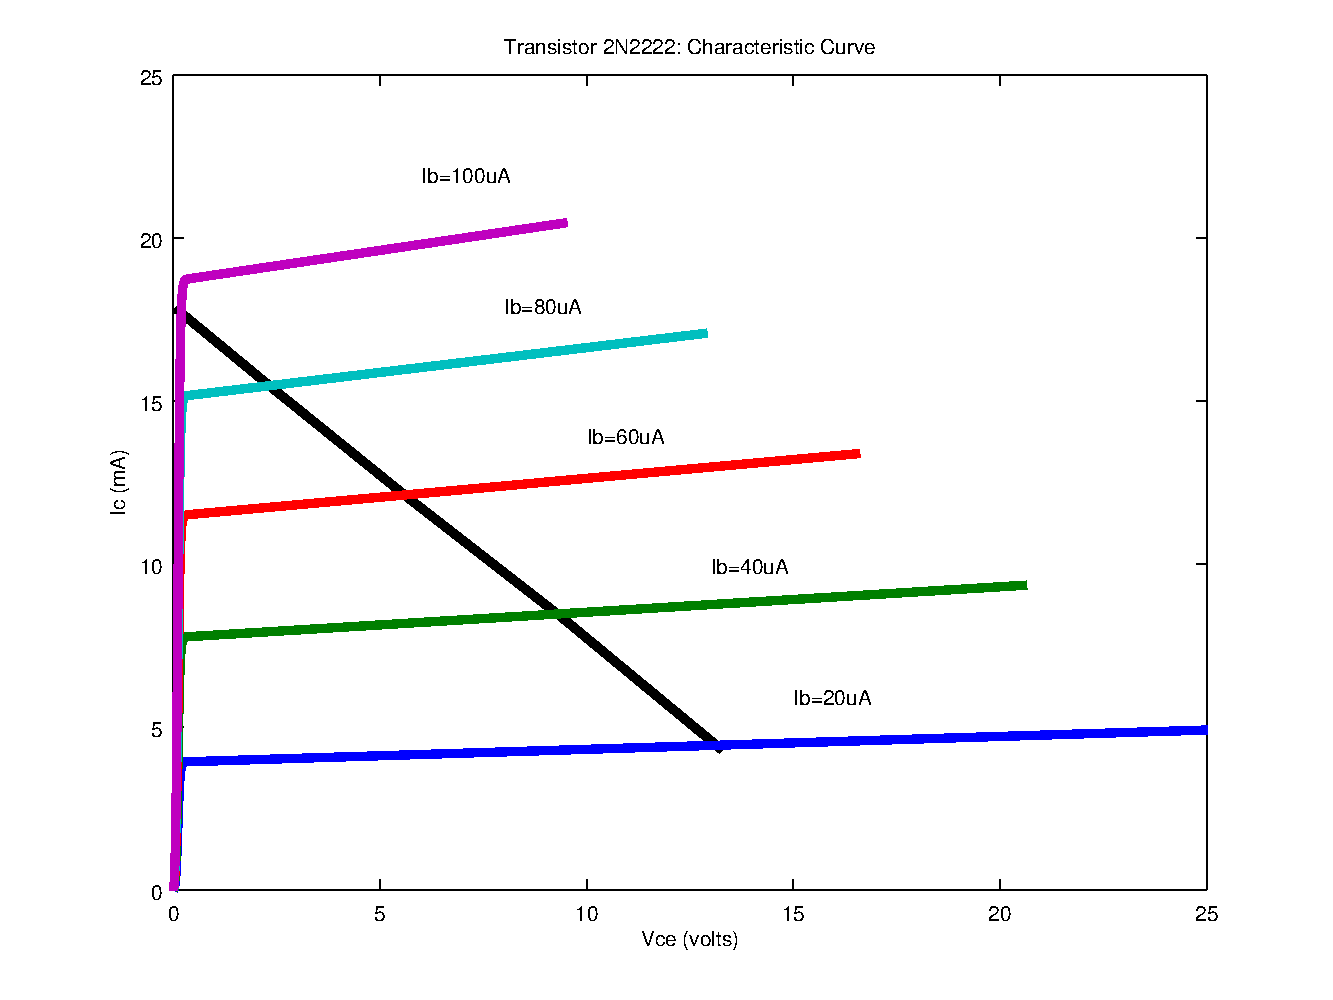
\includegraphics[width = \textwidth]{partHW/TransCharacts2N2222}
	\caption{Transistor Characteristics: NPN 2N2222}
	\label{fig:2N222Chars}
	\end{figure}

	\begin{figure}[h!]
	\centering
	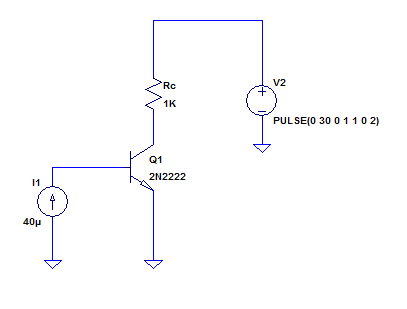
\includegraphics[width = 0.5\textwidth]{partHW/ConstantCurrentSourceBase}
	\caption{CE Amplifier with Constant Current Source and a Varying $V_{CC}$}
	\label{fig:ConstIb_VaryingVcc}
	\end{figure}

\subsection{Effect of $V_{CC}$ and $I_C$ on Current Gain}
We found out earlier that the open loop gain, $A_{OL}$ for 2N2222 transistor is 200. But that was in a specific context - we were using a circuit that had a $1K\Omega$ resistor at the Base, a $1K\Omega$ resistor at the Collector and a $V_{CC}$ of 5V. But what happens when this context changes? Will the current gain remain the same? Let us find out. 

	\begin{figure}[h!]
	\centering
	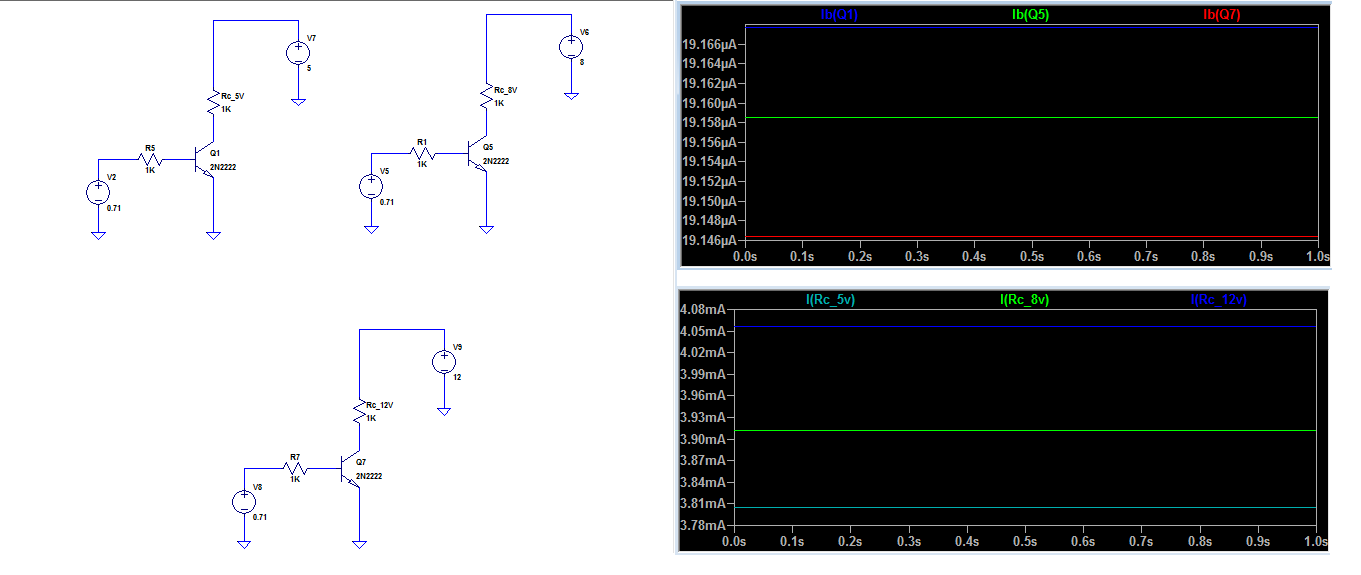
\includegraphics[width = \textwidth]{partHW/betaVsVcc}
	\caption{Effect of $V_{CC}$ value on Current Gain}
	\label{fig:betaVsVcc}
	\end{figure}

\autoref{fig:betaVsVcc} shows three similar circuits with changing $V_{CC}$ value while everything else is the same. It also shows what happens to $I_C$ when $V_{CC}$ is changed. Just to be sure, values of $I_B$ are also plotted. There are several interesting observations from the results:
	\begin{itemize}
	\item Changing $V_{CC}$ had an effect on $I_B$. The effect was small: A 60\% and 140\% change in $V_{CC}$ respectively changes $I_B$ by merely -0.04\% and -0.1\% respectively. 
	\item The effect of $V_{CC}$ on $I_C$ was also small. A 60\% and 140\% change in $V_{CC}$ changed $I_C$ by 2.8\% and 6.8\% only.
	\item Consequently, $A_{OL}$ changes by 3\% and 7\% respectively for $V_{CC}$ changes of  60\% and 140\%  respectively. In other words, changing $V_{CC}$ had an insignificant  effect on the current gain.
	\item The implication of the previous point is that, when $V_{CC}$ changes, $V_{CE}$ is the only quantity affected. 
	\end{itemize}

	\begin{figure}[h!]
	\centering
	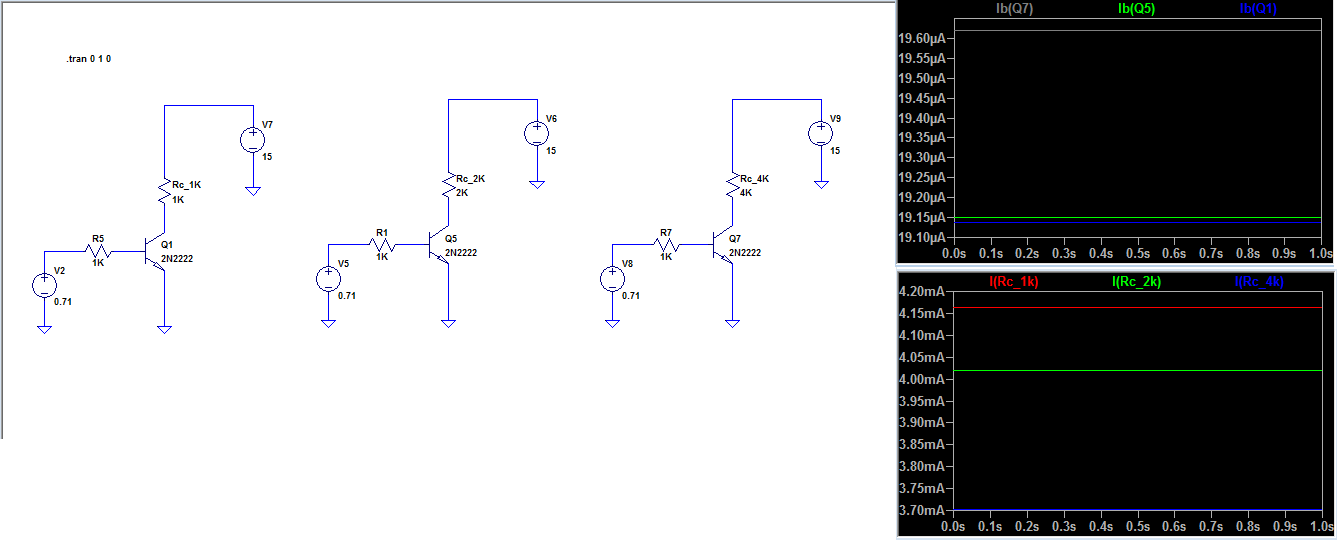
\includegraphics[width = \textwidth]{partHW/betaVsRc}
	\caption{Effect on $R_C$ value on Current Gain}
	\label{fig:betaVsRc}
	\end{figure}

\autoref{fig:betaVsVcc}  shows three similar circuits with changing $R_C$ value while everything else is the same. It also shows what happens to $I_C$ when $R_C$ is changed. Just to be sure, values of $I_B$ are also plotted. There are several interesting observations from the results:
	\begin{itemize}
	\item Changing $R_C$ has negligible effect on $I_B$. A 100\%, 400\% change in $R_C$ values caused a 0.005\% and 2.5\% change in $I_B$ respectively
	\item Same was the case with $I_C$. A 100\% and 400\% change in $R_C$ changed $I_C$ by -3.3\% and -11\% only.
	\item Consequently the effect of changing $R_C$ had an insignificant effect on the $A_{OL}$. A 100\%, 400\% change in $R_C$ values caused a -3.2\% and -13.3\% change in $A_{OL}$ values respectively.
	\item An interesting implication is that, it is important to choose an appropriate $V_{CC}$ for this experiment. For instance, choosing a $V_{CC}$ of 8V instead of 15V would have misled us with the results: Remembering from the previous experiment that changing $V_{CC}$ has practically no effet on $A_{OL}$, and interpreting the result of emph{this} experiment, the value of $I_C$ would have remained at somewhere close to 4mA, resulting in a voltage drop of 8V and 16V across $R_C$ when its values are $2K\Omega$ and $4K\Omega$ respectively. Since the supply itself is 8V, this would have meant that $V_{CE}$ would have been 0V and the drop across $R_C$ in both cases would have saturated to 8V. In other words, we would have driven the transistor into its saturation region.
	\end{itemize}

\section{Amplifier Operating Point and DC Load Line}
When we design an amplifier, it is prudent for us to not expect the input signal to have a DC value of about 0.7V (in the case of a 2N2222 transistor). Firstly it is normal for the person using the amplifier to assume that it will amplify a small signal with a DC value of 0V into a large signal, again centered around 0V DC. Secondly, different transistors will have different operating voltages - It is unfair to impose the requirement of setting the correct DC value for $V_{in}$ on the user. Hence it is advisable to have internal arrangement that will keep the transistor at the so called quescient point or DC operating point that will allow the maximum range of input values a transistor can handle without sacrificing linearity \footnote{It is important to understand that, although biasing a transistor is useful as explained in this paragraph, it is detrimental in circuits where power consumption is the biggest issue. After all, when the transistor is biased. it will have some Base current, and more importantly, some Collector current flowing even when there is no input signal, amounting to wastage of power. Imagine a battery powered device which remains in stand-by state (no input) for a long time, such as a walkie-talkie. Biasing is obviously a bad idea in those cases.One should instead spec out the input signal requirement and meticulously ensure that the circuitry to the left of the transistor is engineered to produce the required type of input signal. For the sake of continuity of the discussions, let us save further discussions on these cases to a later time}.

To start with, we need a way to supply some Base current even when there is no input. The only other power source for the amplifier is $V_{CC}$ and so we obviously have to derive our $I_B$ from it. Besides that, we also need to have a mechanism by which the input signal's voltage gets added to the quiescent voltage at the Base. This can be achieved by using an input capacitor. Finally, the output of the amplifier needs to have a signal with a DC value of 0. This can also be achieved by using a capacitor. So the circuit in \autoref{fig:SimpleBias} represents the starting point for setting up our CE amplifier's quiescent point. 

	\begin{figure}[h!]
	\centering
	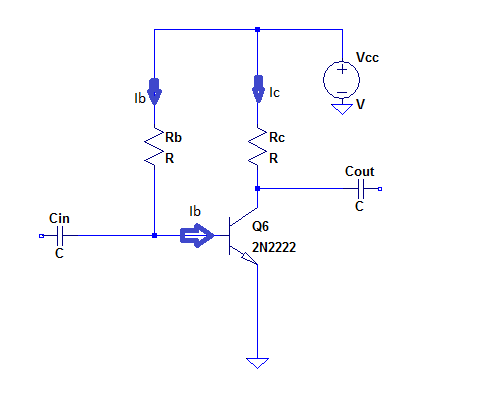
\includegraphics[width = 0.5\textwidth]{partHW/SimpleBias}
	\caption{CE Amplifier with Constant Current Source and a Varying $V_{CC}$}
	\label{fig:SimpleBias}
	\end{figure}

From this circuit, one can draw two equations as shown below:
           
           \begin{align}
	V_{CC} - I_B*R_B - V_{BE} = 0 \label{eq:BEloop1} \\
 	V_{CC} - I_C*R_C - V_{CE} = 0 \label{eq:CEloop1}
	\end{align}

With these two equations, we can solve two unknowns - often, they are $R_B$ and $R_C$. In other words, we will have to come up with some values for the other variables in the equations and then solve the equations to find out $R_B$ and $R_C$. Among the variables we need to fix, $V_{CC}$ is often a system-level constraint. For example, it may be battery operated system using two AA batteries, in which case, the $V_{CC}$ will be <6V. Once $V_{CC}$ is available, next step is to decide how much the max value of $I_C$ should be. Power consumption constraints, load's ability to handle current if $R_C$ itself is the load, the max current capacity of the power source, circuit heat requirements etc. will determine $I_{Cmax}$. We can then draw the DC load line in \autoref{fig:2N222Chars}. Note that, since $I_C = I_{Cmax}$ when $V_{CE} = 0$, using \autoref{eq:CEloop1}, one can directly find $R_C$ value. Or, one can also determine quiescent point $V_{CE}$ and $I_C$ values first and then substitute them into \autoref{eq:CEloop1} to find $R_C$. Both methods will give the same $R_C$ value. Deciding what quiescent $V_{CE}$ should be will depend on standby power requirements and/or expected input signal range (and hence the expected signal output range). If range is the concern, then it makes sense to choose quiescent $V_{CE}$ to be $\frac{V_{CC}}{2}$. Since the transistor always operates along the DC load line, once quiescent $V_{CE}$ is chosen, quiescent $I_C$ and $I_B$ assume consequential values. Besides these, from \autoref{fig:VbeIbVsVin}, $V_{BE}$ can be found out for a given $I_B$ value. Thus, we will have all the information available with us to find $R_B$ using \autoref{eq:CEloop1}. 

\subsection{Example}
Let us assume that $V_{CC}$ is 6V and $I_{Cmax}$ is 6mA. That would meant that $R_C$ should be $1K\Omega$. Now the DC load line equation can be obtained by observing that the end points are ($V_{CC}$, 0) and (0, $I_{Cmax}$):

	\begin{align}
	\frac{y - 0}{I_{Cmax}} &= \frac{x - V_{CC}}{-V_{CC}} \\
	Rearranging., \\
	y &= \frac{-I_{Cmax}}{V_{CC}} * x + I_{Cmax} \label{eq:dcLoadLine}\\
	   &= \frac{-1}{R_C} * x + I_{Cmax} \label{eq:dcLoadLineAlter}\\
	\end{align}

So, if we choose quiescent $V_{CE}$ to be $\frac{V_{CC}}{2}$, then using equation \autoref{eq:dcLoadLine}, we find out that quiescent $I_C$ will be 3mA. Since 2N2222 has a current gain, $A_{OL}$ of 200(approx), that would mean that $I_B = 15\mu A$.  For this $I_B$, $V_{BE}$, from \autoref{table:VbeVsIb} is approximately 0.685V. Substituting these in equation \autoref{eq:BEloop1},

	\begin{align}
	R_B &= \frac{V_{CC} - V_{BE}}{I_B} \\
	       &= \frac{6 - 0.685}{15\mu} \\
	       &= \frac{5.315}{15\mu} \\
	       &= 354.33 K\Omega
	\end{align}

We can substitute the above values in a SPICE model and verify using simulations that we are indeed achieving the quiescent point values for $I_C$ and $V_{CE}$ as desired. But in the real world, all resistor values aren't available\footnote{Unless we are talking about a custom designed LSI circuit}. So we will have to choose a popular resistor whose value comes the closest to the $R_B$ value of $354.33 K\Omega$.This happens to be $330K\Omega$. Using this $R_B$ value, we can either reverse engineer $V_{BE}$, $I_B$ combination using \autoref{table:VbeVsIb} - In a way, we used the above calculations to get an idea of the $R_B$ value we are looking for, and then work our way backwards to find out what $I_C$ is going to be. We can then, if desired, tweak the $R_C$ value to come up with something that will get us closer to the quiescent $V_{CE} = \frac{V_{CC}}{2}$ point. We can use maths for all this or simply run simulaitons with $330K\Omega$ of $R_B$ and play with $R_C$ values. I used simulations to find out that $I_C$ will be 3.25mA. So if we desire a $V{CE}$ of $\frac{V_{CC}}{2}$, then our $R_C$ should be $\frac{3V}{3.25mA} =  923\Omega$. So if we can find a resistor value closer to $923\Omega$ than $1K\Omega$ is, then we can use that resistor instead of a $1K\Omega$ resistor for $R_C$.

\emph{A note on the input dynamic range}: For a moment, let us assume that we don't get a resistor value closer to $923\Omega$ than $1K\Omega$ is. At $R_C = 1K\Omega$, our quiescent $V_{CE}$ is already at 2.747V. We can only go down to 0V\footnote{Had our calculations gave us an $I_C$ such that quiescent $V_{CE}$ ended up being higher (instead of lower) than $V_{CC}/2$, then the upper limit of 6V (i.e., $V_{CC}$ would have been more restrictive on the $V_{CE}$ swing than the ground level of 0V}. This means that, on the lower side, we have a room of 2.747V instead of a desired swing of 3V with which we set out our design. Since our input signal is very likely to have an equal swing on the positive and negative side, this implies that the $V_{CE}$ value cannot swing more than 2.747V, not only on the negative side but also on the positive side as well. So the max value of $V_{CE}$ will be $2.747V + 2.747V = 5.494V$. To achieve this $V_{CE}$, we need a drop of $6V - 5.494V = 0.506V$, in other words, an $I_C$ of $0.506 mA$. Since our $A_{OL}$ is approximately 200, this would mean an $I_B$ of $2.53\mu A$, or, referring to {table:VbeVsIb}, a $V_{BE}$ of 0.637V. Our quiescent $V_{BE}$ is 0.686V (found from simulation). This leaves us a room of $0.686V - 0.637V = 0.049V$. In other words our input signal's maximum allowed swing is 100mV (approx).

It is always important to check in simulation if our theoretical calculations are right. This is because we have made some simplifications related to linearlity between $V_{BE}$, $I_B$ and more that are not a 100\% true in reality. Furthermore, we also have deviated from theoretical values (ex. $R_B$ value). So \autoref{fig:VccDerivedIqEx} shows the simulation results of our actual circuit.

	\begin{figure}[h!]
	\centering
	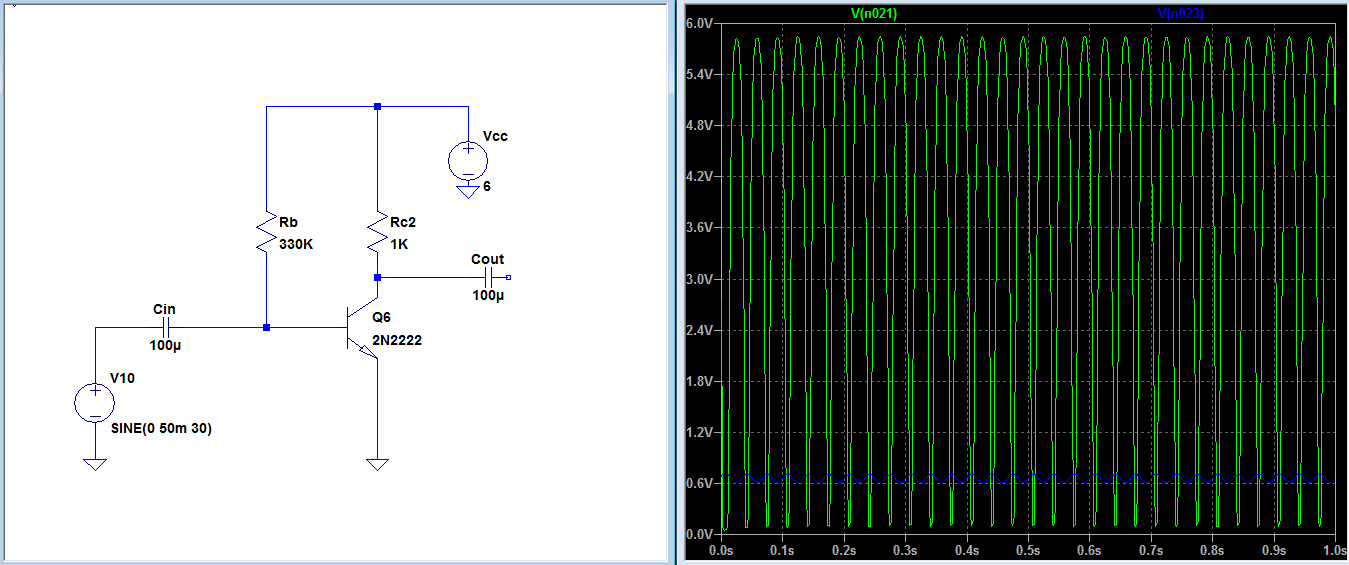
\includegraphics[width = \textwidth]{partHW/VccDerivedIq}
	\caption{CE Amplifier with DC biasing derviced from $V_CC$}
	\label{fig:VccDerivedIqEx}
	\end{figure}

We can clearly see that the $V_{CE}$ signal is covering the entire voltage range possible - so our prediction that the input signal swing can't be more than a 100mV was right.

%\subsection{Thermal Runaway}
%
%\subsection{Collector Derived Biasing}
%To avoid thermal runaway, one can use a biasing as shown in \autoref{fig:collectorDerivedIq}. 
%
%	\begin{figure}[h!]
%	\centering
%	\includegraphics[width = \textwidth]{partHW/collectorDerivedIq}
%	\caption{CE Amplifier with DC biasing derviced from $V_CC$}
%	\label{fig:collectorDerivedIqEx}
%	\end{figure}
%
%The Collector to Base connection represents a negative bias. If $A_{OL}$ increases in the quiescent state, it will increase $I_C$, which will decrease $V_{CE}$. This will reduce $I_B$, thus maintaining the quiescent $I_B$, $I_C$ values. The following are equations corresponding to this circuit.
%
%	\\begin{align}
%	V_{CC} - I_C*R_C - I_B*R_B - V_{BE} = 0 \label{eq:collectorDerivedIq_baseLoop} \\
%	V_{CC} - I_C*R_C - V_{CE} = 0 \label{eq:collectorDerivedIq_emitterLoop} 
%	\\end{align}
%
%As before, we will likely know our $V_{CC}$, quiescent $I_C$, $V_{BE}$ and $V_{CE}$ values. We will use them in \autoref{eq:collectorDerivedIq_baseLoop} and \autorefl{eq:collectorDerivedIq_emitterLoop}
%
%
%\section{Topics to Talk About}
%	\begin{itemize}
%	\item How $A_{OL}$ changes with input frequency. 
%	\end{itemize}






\begin{thebibliography}{9} % Support up to 9 references

\bibitem{sanghoKim16} 
  Sangho Kim,
  \href{https://www.youtube.com/watch?v=7ukDKVHnac4}{\emph{Transistors, How to they Work?}},
  Learn Engineering, Massachusetts,
  2nd edition,
  2016.

\end{thebibliography}
%\chapter{Analog Electronics}
%\section{Amplifier}
%Real-life amplifiers are very different from ideal amplifiers in that,
%	\begin{itemize} 
%	\item Their gain decreases with increasing frequency
%	\item Their gain changes with temperature
%	\item They do add noise
%	\item They don't have a linear response at all input amplitude levels
%	\end{itemize}
%
%The limited linearity problem is taken care of by properly biasing the amplifier. Their gain variation due to temperature is taken care of by using a negative feedback. There is nothing one can do about the noise and the non-flat frequency response. 
%
%\subsection{Negative Feedback for Gain Stability}
%Suppose an amplifier gain (open loop gain) is $A_0$. So $V_{out} = A_0.V_{in}$. But now consider a negative feedback as shown below.
%	\begin{figure}[h!]
%	\centering
%	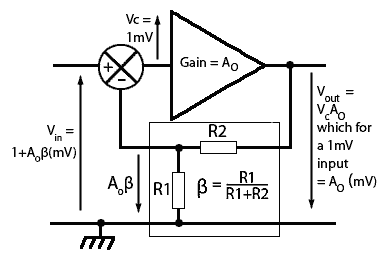
\includegraphics[width = 0.5\textwidth]{partHW/NegFeedbackAmplifier}
%	\caption{Closed Loop Amplifier}
%	\label{fig:clAmp}
%	\end{figure}
%
%Now, let us calculate the closed loop gain:
%	\begin{flalign*}
%	V_{out} &= A_0.V_c	 \\
%	V_{out} &= A_0(V_{in}-V_{out}*\beta)	 \\
%	\frac{V_{out}}{V_{in}} &= \frac{A_0}{1+A_0\beta} 
%	\end{flalign*}
%When $A_0\beta$ is large, which is usually the case because $A_0$ is large, then the transfer function can be simplified to $\frac{1}{\beta}$. This means that, the amplifier closed loop gain is independent of its open loop gain $A_0$ and completely dependent on the values of resistor $R_1$ and $R_2$. This is good news as the open loop gain of an amplifier varies widely as temperature changes, whereas resistance values of resistors hardly change with temperature. Thus a closed loop amplifier has a much more stable.
%
%\subsection{Oscillator}
%Oscillator is essentially an amplifier with a positive feedback for just one frequency\marginnote{Oscillator is amplifier with positive feedback for one frequency}. This is achieved by using a bandpass filter at the output of an amplifier to filter out a select frequency which is then fed back as the input of the amplifier. Electronic noise inherent in the amplifier acts as a seed. Since electronic noise is usually white, it contains all frequencies, out of which the BPF selects one (actually a narrow band). It is important to remember that the feedback must be positive - for that, the frequency fed back must be in-phase with the input of the amplifier. Remember that the amplifier itself contributes to a phase diff between the input and the output and the BPF may add to it. It is entirely possible that the BPF may peak at a frequency, but its phase response at that frequency isn’t right to make the loop phase response to be 360 degrees. In that case, some other frequency, whose phase shift is just right could become the oscillating frequency, even though the BPF magnitude response may be much smaller at that frequency.
%
%The following diagrams show two practical oscillator designs, the left one at 10.5 KHz and the right one at 2 KHz.
%	\begin{figure}[h!]
%	\centering
%	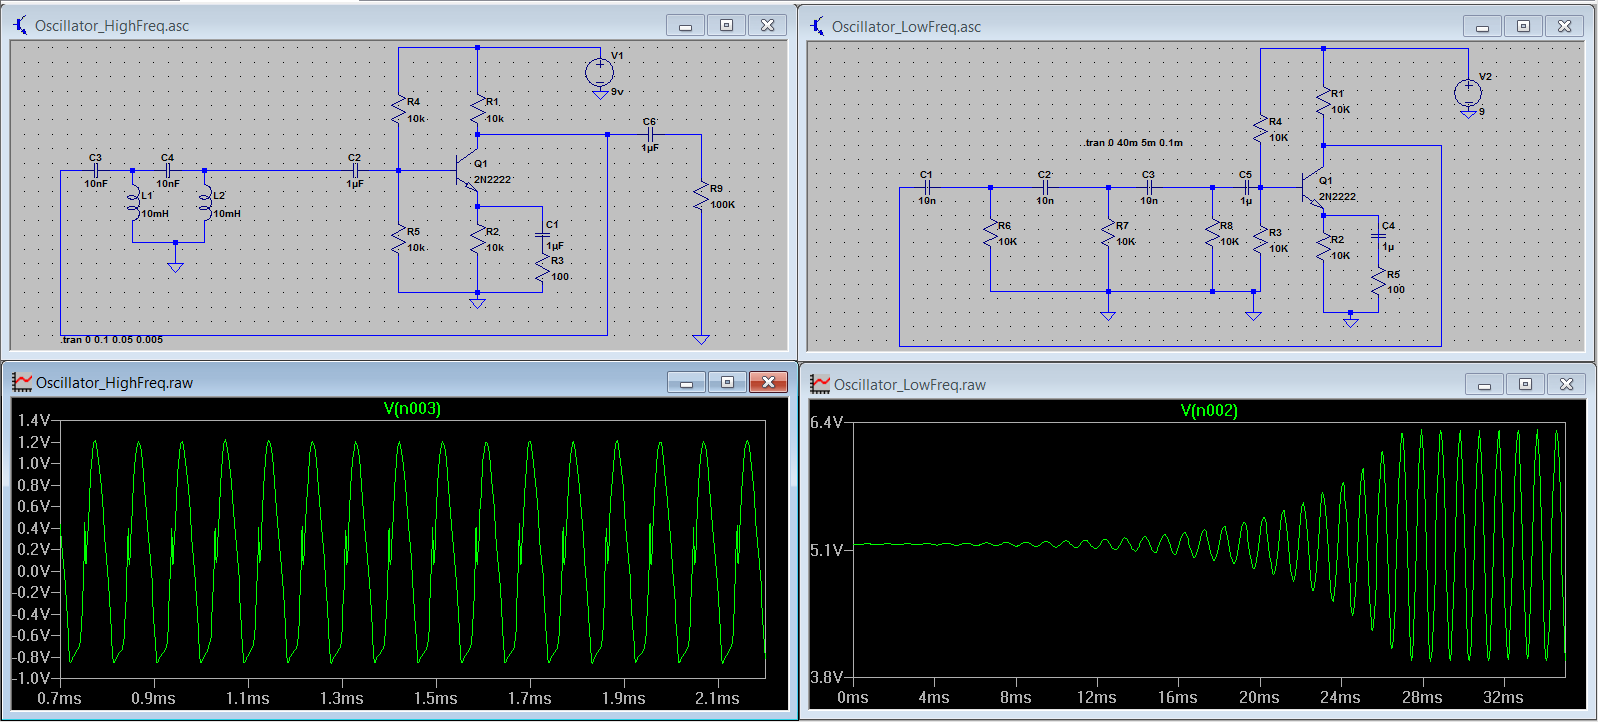
\includegraphics[width = \textwidth]{partHW/Oscillators}
%	\caption{Oscillator Designs}
%	\label{fig:oscs}
%	\end{figure}
%
%Remember that the BPF and anything else attached to the output of the amp contributes to the output impedence and hence has an effect on the amplifier gain. This could be a problem when the BPF needs to center at a very high frequency which will typically lead to small R, C, L values which may reduce the output impedence. 






	

